%!TEX program = xelatex
% 完整编译: xelatex -> bibtex -> xelatex -> xelatex
\PassOptionsToPackage{table,xcdraw}{xcolor}
\documentclass[lang=cn,12pt,a4paper,cite=authoryear]{elegantpaper}

\title{基于文本分析和网络分析的\\德国铁路列车延误数据挖掘}
\author{经71 肖昌荣 \\ 2017012527}
\institute{清华大学经济管理学院}

%\version{0.09}
\date{\zhtoday}


% 本文档命令
\usepackage{array}
\newcommand{\ccr}[1]{\makecell{{\color{#1}\rule{1cm}{1cm}}}}
\usepackage{booktabs}
\usepackage{float}
\linespread{1.5}

\begin{document}

\maketitle

\begin{abstract}
本文旨在控制德铁列车晚点现象,减少德铁公司的运营成本并提高德铁列车乘客的服务体验,对德国铁路一天内正常和晚点列车的数据进行分析。首先在车站、列车类型和一天内的时间段三个角度对数据集进行切块处理,分析列车总流量、晚点列车数量、延误时长等指标在不同角度呈现出的特点。接着使用分词、统计词频、构建词云等文本分析技术,提取主要的晚点原因。然后使用加工后的数据构建列车总流量、晚点总时长的交通网络图,利用网络分析方法中的中心性作为指标衡量车流量及延误情况,进一步构建动态交通网络,探究一天内不同时段的交通流特点。通过上述分析,作者发现数据的诸多隐藏特点,并结合假定的心智模型提出具有现实指导意义的管理启示,点明可能的进一步研究方向,对德国铁路公司(Deutsche Bahn AG)和未来研究相关问题的学者有指导和借鉴意义。
\keywords{列车晚点,文本分析,网络分析}
\end{abstract}

\newpage

\tableofcontents

\newpage

\section{前言}

德国铁路股份公司(Deutsche Bahn AG)一般简称为德国铁路(DB),是一家总部设于柏林的德国国有运输公司,于1994年在法兰克福创立,由原德国联邦铁路及德国国营铁路合并而成。目前,它是仅次于德国邮政的世界第二大运输企业,也是欧洲最大的铁路运营商及铁路基建商\citep{DB_wiki}。

\cite{DB_joke}在2018年报道,尽管德国人和德国企业一向以认真严谨的态度享誉世界,曾同样以这种精神为招牌的德国铁路,却因为现实中经常发生的长时间晚点、列车班次取消等状况为人诟病与调侃。列车晚点现象无论对德国铁路还是顾客都带来了很大的影响。对于顾客的影响显而易见,晚点很可能打乱顾客的后续安排,例如因为前一趟列车的晚点而赶不上换乘列车等。对于德国铁路,列车经常性的晚点会对后续列车造成影响,也可能为运营者的列车进站轨道站台的排程带来麻烦,增加服务台的工作量;同时,如上文所提及的,晚点现象会降低铁路运营公司的商誉,使得顾客不再信任该公司的列车服务。在这一点上德铁的处理较为妥当,如果因为列车晚点而错过换乘,则可以在服务台无条件改签为下一班;若晚点时间超过一小时,可以填写反馈表来获得损失补偿。但无论如何,列车晚点对于德国铁路都是一笔不小的成本,在2018年德铁就因为列车晚点问题支付了5300万欧元的乘客补偿\citep{DB_cost}。

\begin{figure}[H]
	\centering
	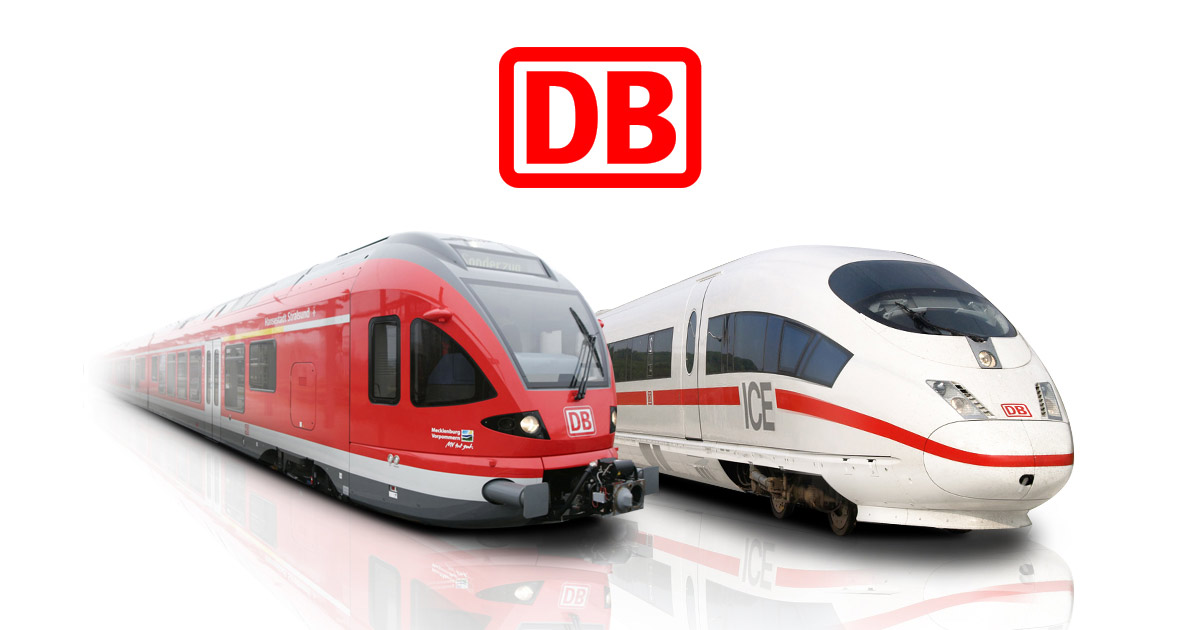
\includegraphics[width=0.8\textwidth]{image/DB1.jpg}
	\caption{德国铁路公司标志及代表列车型号}
	\label{fig0}
\end{figure}

所以本文将针对德国铁路列车晚点这一问题,根据德国各大车站某天正常运行列车与晚点列车的信息数据,观察晚点数据特点,分时段对列车数据进行分析,发现其中的规律及列车晚点的主要原因。我们以德铁运营公司的角度,利用本文数据集中的已知信息,适当结合生活经验,\textbf{将控制德铁列车晚点现象、减少德铁公司的运营成本并提高德铁列车乘客的服务体验作为心智模型},把问题细分为列车自身技术问题、列车线路问题、车站排程问题等多个子问题,尝试提出在运营管理中可能的改进方案,减少因晚点带来的不必要的损失。

在文章接下来的部分,我们首先简单介绍分析所使用的数据集,对数据进行描述性统计分析,通过图表的直观形式发现数据的特点。接着摘取列车晚点原因,使用文本分析手段获得列车晚点的主要原因。然后根据列车在各个车站之间的交通,建立静态和动态的网络模型,使用网络分析方法挖掘更多有价值的信息。最后,总结归纳出有实际意义的管理启示。


\section{数据简介}

本文的数据集选自Kaggle网站用户摘取整理好的德国铁路列车信息数据,原作者是从德国铁路官网爬取相关信息,数据来源详见链接:\url{https://www.kaggle.com/chemamengibar/dbahn-travels-captures/data}。

数据集为2019年6月20日当天,经过Berlin, Bremen, Dresden, Frankfurt, Hamburg, Hannover, Köln, Mainz, Müchen, Stuttgart十个德国主要车站的列车信息。数据集按照城市分为\textbf{10个csv文件,每个文件大致3万条记录,合约35万条}。每个文件中的数据有如表(\ref{tab1})所示的内容:

\begin{table}[H]
	\centering
	\caption{数据集内容简介}
	\label{tab1}
	\begin{tabular}{lll}
		\hline
		\multicolumn{1}{c}{名称} & \multicolumn{1}{c}{数据类型} & \multicolumn{1}{c}{解释}  \\ \hline
		TAA                    & 字符串                      & 列车晚点原因。                 \\
		TA                     & 字符串                      & 实际离站时间。                 \\
		TIN                    & 字符串                      & 列车型号。                   \\
		TIR                    & 字符串                      & 列车行驶路线。                 \\
		TSI                    & 字符串                      & 车站编号。                   \\
		TIM                    & 布尔值                      & 列车行驶方向,arr表示到达,dep表示离开。 \\
		TIRE                   & 字符串                      & 列车行驶目的地。                \\
		TIP                    & 字符串                      & 站台号。                    \\
		TIT                    & 字符串                      & 预计离站时间。                 \\
		TID                    & 字符串                      & 日期。                     \\
		TSC                    & 字符串                      & 车站名称及编号。                \\
		TAc                    & 整数值                      & 延误时间,TAc=TA-TIT,单位分钟。   \\ \hline
	\end{tabular}
\end{table}

其中数据既包含正常运行的列车信息,也包含晚点列车信息,所以正常列车记录的晚点原因、延误时间等属性为空,我们以此来判断某条记录为正常列车或是晚点列车。

德铁的列车主要分为ICE、IC、RE、S、EC几种,具体如下:
\begin{itemize}
	\item ICE(Inter City Express),即城际特快,是德国境内最快的车,可类比于中国的高铁动车,主要在大城市大车站停,通往其他国家的列车多为ICE。
	\item IC(Inter City),即城际快车,相比ICE车速较慢,但停靠的站点更多。
	\item RE(Regional Express),即地区特快,在一个州/地区内较小的城市都会停靠。
	\item S(Stadtbahn),即城市列车,类似地铁或有轨电车,是城市内连接至火车站的交通方式。
	\item EC(Euro City),即欧洲城市列车,也是快车的一种,不只在德国境内运行,而是连接了很多欧洲的大城市。
\end{itemize}

数据中混有数据集创建者爬取数据时产生的爬取错误提示,同一趟列车的晚点信息也经常出现被多次爬取的情况。所以在数据清洗过程中我们将其作为无效数据去除,处理后的数据集约有17万条记录。在下一部分,我们将对数据进行更为详细的介绍分析。

\section{数据特点统计分析}

\subsection{各车站间对比}

首先观察各个车站当天的总车流量和晚点列车数,如下图(\ref{fig1})所示。

\begin{figure}[H]
	\centering
	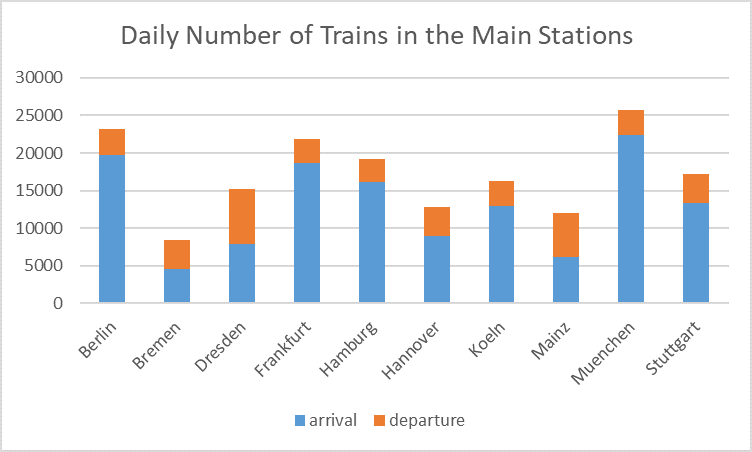
\includegraphics[width=0.45\textwidth]{image/num.png}
	\quad
	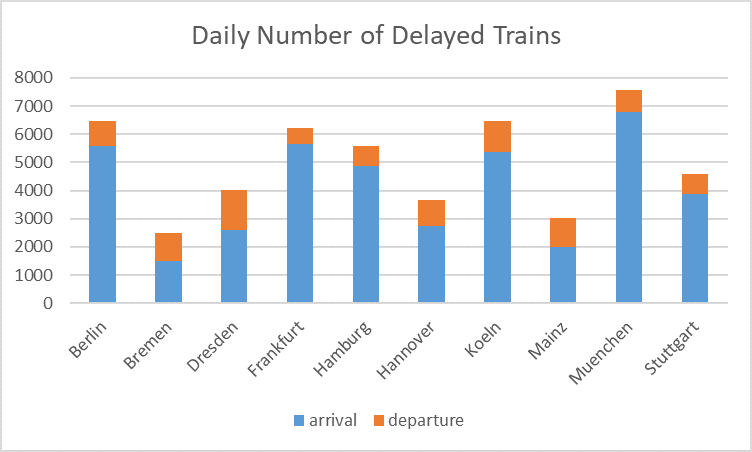
\includegraphics[width=0.45\textwidth]{image/delay_num.png}
	\caption{各车站总车流量及晚点列车数}
	\label{fig1}
\end{figure}

我们发现,比起从车站出发的列车,\textbf{到达车站的列车占车流量的绝大部分},这是因为我们选取的都是主要火车站,每个车站所处地区都有许多城内、地区内的列车向主火车站汇总。\textbf{总车流量相对较多的是柏林、法兰克福、慕尼黑}车站,这些车站都是地区和长途的交通枢纽,数据所展示的与现实情况相符。同时,各车站晚点列车数量所占总车流量的比例也基本相同,即各车站总车流量的相对多少,基本能够反映其晚点列车数量的相对多少。

\begin{figure}[H]
	\centering
	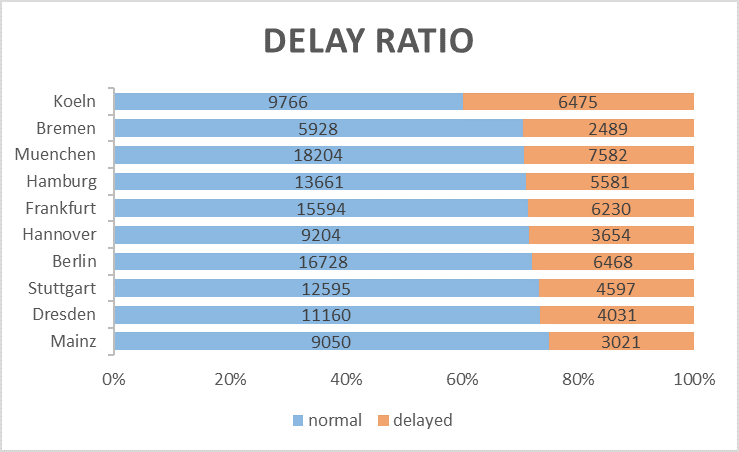
\includegraphics[width=0.6\textwidth]{image/delay_ratio.png}
	\caption{各车站晚点列车比例}
	\label{fig2}
\end{figure}

接着我们计算出各个城市的列车晚点率,如图(\ref{fig2})所示。发现与我们之前的判断大致相符,各个车站的晚点率在$25\%$至$30\%$之间,\textbf{其中科隆的晚点率最高,达到了约$39\%$}。我们发现车流量大的大车站晚点率会相对更高,这也许是因为这些大车站有更多的长途甚至国际列车,更有可能发生晚点事件,例如地处德国西北部的科隆是德国通往比利时、荷兰、卢森堡等国的枢纽,几乎所有从这一方向出德国国境的ICE列车都要经过科隆。

而对于每趟晚点列车的平均晚点时间,\textbf{法兰克福远高于其他车站,达到了约8分钟},结果如图(\ref{fig3})所示。

\begin{figure}[H]
	\centering
	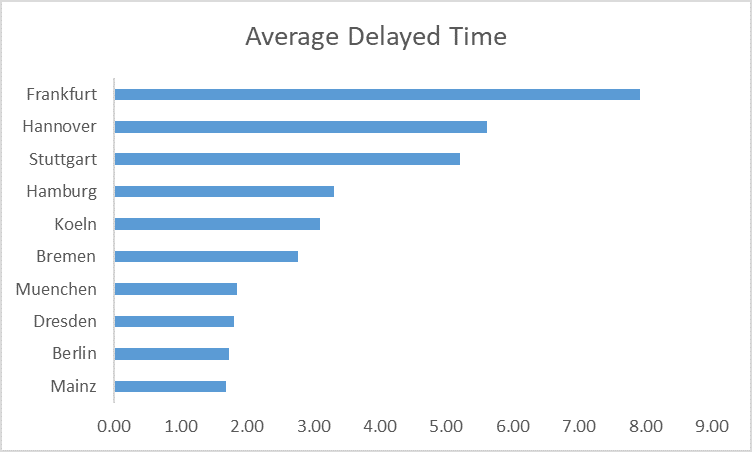
\includegraphics[width=0.6\textwidth]{image/avg_time.png}
	\caption{各车站平均每趟晚点列车的延后时长}
	\label{fig3}
\end{figure}

\subsection{各时间段间对比}

我们猜测列车车流量与列车晚点数会在一天中不同时间段发生变化,于是将数据按小时分为多个时段。然而,由于原始数据爬取的缺失,以及凌晨时段到达列车数过少,我们最终将数据划分为从早晨11时至夜晚23时这13个时段,依此进行分析。下图(\ref{fig4})是数据集中所有车站的总体概况。

\begin{figure}[H]
	\centering
	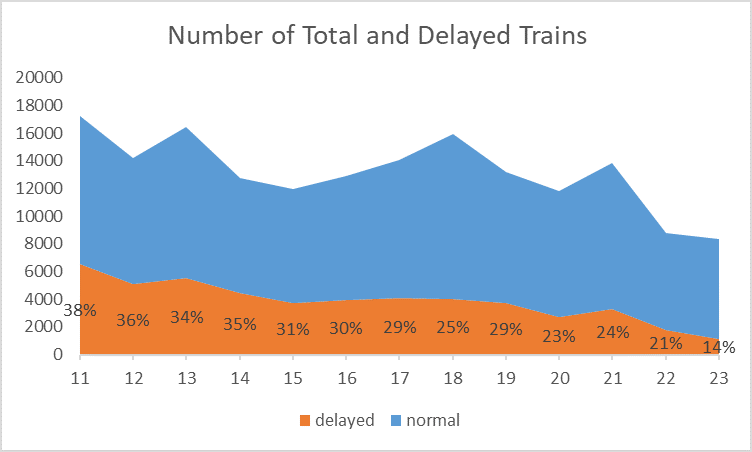
\includegraphics[width=0.6\textwidth]{image/time_total.png}
	\caption{各时段总车流量与晚点列车数量概览}
	\label{fig4}
\end{figure}

从图中我们不难发现,\textbf{车流主要有中午11时、13时及晚间18时、21时四个高峰},且整体有着\textbf{随时间推移而递减}的趋势。晚点列车数量有类似的高峰时段,但与总车流量相比高峰幅度不大,只在中午时间的两个高峰较为明显,总体较为平缓。对于列车晚点率,则有更加明显的随时间递减的趋势,特别是在深夜23时后降到了约$14\%$。

接下来我们选取几个更有特点的主车站进行观察。法兰克福车站几乎完美契合整体的车流量趋势,在中午11时、13时及晚间18时、21时有明显的四个高峰,同样拥有这种规律的还有柏林、科隆主火车站;而慕尼黑则不同,中午11时有一个十分明显的高峰,但13时的车流量与12时接近,晚间18时、21时有高峰现象,但相比而言不是很明显,各时间段的数值详见下图(\ref{fig5})。

\begin{figure}[H]
	\centering
	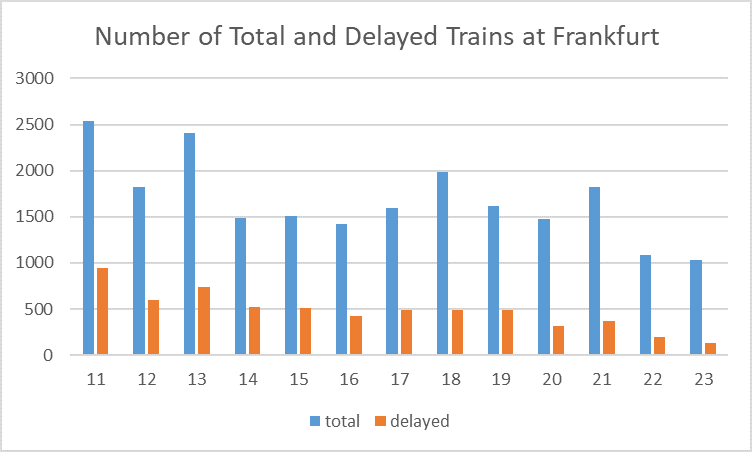
\includegraphics[width=0.45\textwidth]{image/frankfurt.png}
	\quad
	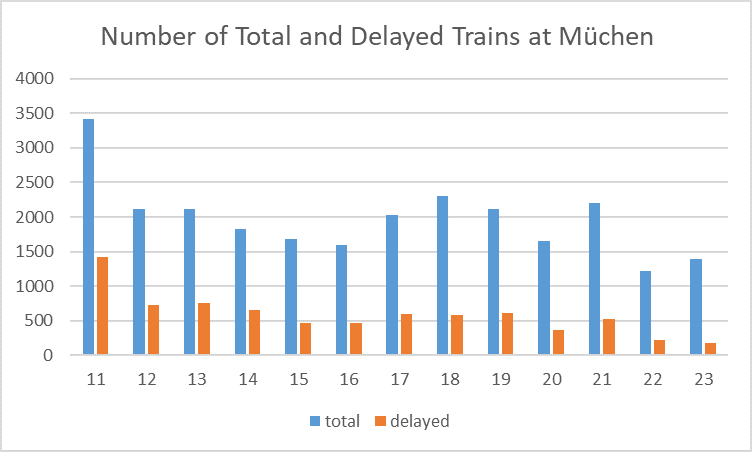
\includegraphics[width=0.45\textwidth]{image/muechen.png}
	\caption{法兰克福与慕尼黑各时段总车流量与晚点列车数量}
	\label{fig5}
\end{figure}


\subsection{长途列车与短程列车对比}

前文介绍了德铁公司列车的主要类型,我们接下来就将探究不同类型列车的晚点情况是否会有所不同。根据现实生活中的经验,我们只考虑I、S、R三种类型的列车,其他非主流列车型号数量较少,对分析的影响可以忽略不计。I类即Inter City,指长途的城际列车,主要连通各大城市,包括ICE、IC等型号的列车;S类即Stadtbahn,指城市内的列车,该种列车每天的班次极多,占数据集中列车记录的一半以上;R类即Regional,指地区列车,功能介于I类与S类列车之间,多为同一地区/省份大小城市之间的交通。

通过观察数据集,我们发现经过这十个主要火车站的\textbf{I类列车数量级在1000次以内,为三类中最少,R类列车次之,S类列车的班次最多},其中慕尼黑的S类列车记录\textbf{超过2万条},占数据集中慕尼黑列车记录总数的近$80\%$。尽管数据有些令人吃惊,但三种列车之间数量级的关系是没有违背常理的,城市内电车、地铁的班次确实是远远高于高铁的途经次数。

图(\ref{fig6})为各车站不同种类列车的晚点率,我们发现S类和R类列车的晚点率与未分类时整体的晚点率相差不大,大致在$30\%$到$40\%$的区间内,但\textbf{I类列车的晚点率却出奇地高},基本都超过了$50\%$。这是因为I类列车为长途的城际列车,运行期间更有可能出现各种导致晚点的情况,而且按照本文的算法,即使晚出发1分钟也会被算作晚点,而对于I类列车来说,数小时的总行程要保证如此的到站精度着实不易,所以使得I类列车的晚点率如此之高。

\begin{figure}[H]
	\centering
	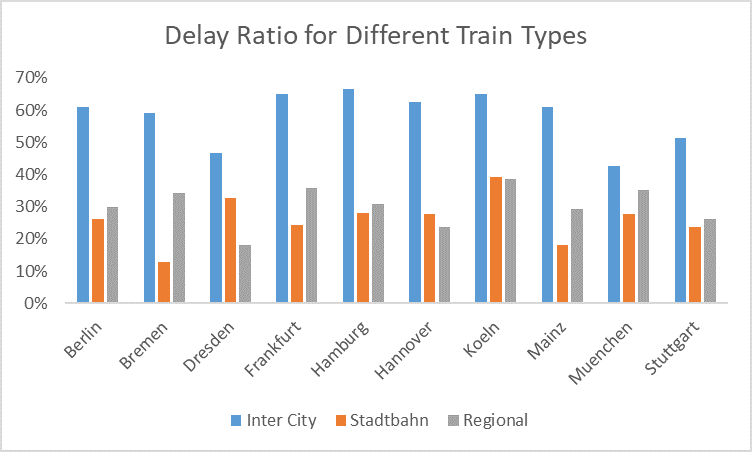
\includegraphics[width=0.6\textwidth]{image/ratio_type.png}
	\caption{各车站不同种类列车的晚点率}
	\label{fig6}
\end{figure}


\section{列车晚点原因分析}

数据集中还包含了列车晚点时德铁在官网中给出的晚点原因,于是我们尝试使用文本分析方法,提取其中有价值的文字信息,发掘列车晚点的主要原因。

\subsection{晚点原因语句分析}

首先使用Python将数据集中所有车站文件中的所有晚点原因摘出,其中部分晚点列车没有给出晚点原因,所以最终得到的晚点原因数量会比晚点列车记录总数少。接着将德语的晚点原因用Google Translate翻译为中文,由于翻译软件有时无法得知句子的具体情境,存在一些晚点原因翻译不够准确的现象,例如"Gleiswechsel"本应是“轨道改变”,却被翻译为“追踪改变”;"Gleis"在本文情景下翻译为“列车轨道”更合适,而不是Google翻译的“赛道”。为了方便理解,后文分析时所采用的都是人工校正后的翻译结果。统计不同原因的频数,频数最高的10条原因如下所示:

\begin{table}[H]
	\centering
	\caption{列车晚点原因出现频数}
	\label{tab2}
	\begin{tabular}{@{}lc@{}}
		\toprule
		\multicolumn{1}{c}{晚点原因} & 出现次数 \\ \midrule
		原因:前面的火车晚点               & 2453 \\
		原因:轨道变化                  & 827  \\
		原因:由于前一次旅行而延误            & 752  \\
		原因:运营延迟                  & 458  \\
		原因:进/出延迟                 & 428  \\
		原因:等待另一列火车的乘客            & 402  \\
		原因:轨道上的人                 & 401  \\
		原因:火车上的技术故障              & 377  \\
		原因:大修                    & 326  \\
		原因:警方调查                  & 291  \\ \bottomrule
	\end{tabular}
\end{table}

可以看出,\textbf{“前面的火车晚点”}这一原因出现的次数为2453,是其他原因的至少3倍以上!同时,\textbf{“由于前一次旅行而延误”}的频数位列第三,它是指列车由于某事件使其在下一站晚点,而之后列车线路上的所有站台也将受此影响而晚点。出现次数第二多的\textbf{“轨道变化”}其实可以理解为其他晚点原因导致的后果,例如,若前面的火车晚点,该火车原先的进站站台被占据,所以可能改变轨道停靠在其他站台,这与“运营延迟”、“进/出延迟”类似,是德铁运营时站台排程改变所引起的。当然,也不排除轨道变化是由于某些事件而临时改变列车线路的情况。还有其他的“技术故障”、“大修”、“警方调查”也都是现实生活中常见的情况。

\subsection{晚点原因词语分析}

由于数据集中的晚点原因都是句子的形式,我们进一步将其细分为词语和短语,尝试发现新的特点。使用Python的jieba包对晚点原因文本进行分词处理,过程中的停词(stopwords)设置为网络下载的常用中文停词库。同时,\textbf{根据该问题的具体情境,将时常出现但对分析没有实际意义的词语作为停词略去},例如“原因”、“火车”、“ICE”、“延误”等,因为数据集描绘的就是火车延误的原因,所以上述词语出现次数必然很多,却并不会对分析起到帮助;而例如“乘客”等词语看似同属于停词,但它表明列车晚点可能是因为车中乘客突发疾病所引起的,具有实际意义,所以不可以作为停词删去。记录每个分词后词语出现的频数,其中出现频数最高的20个词语为:

\begin{figure}[H]
	\centering
	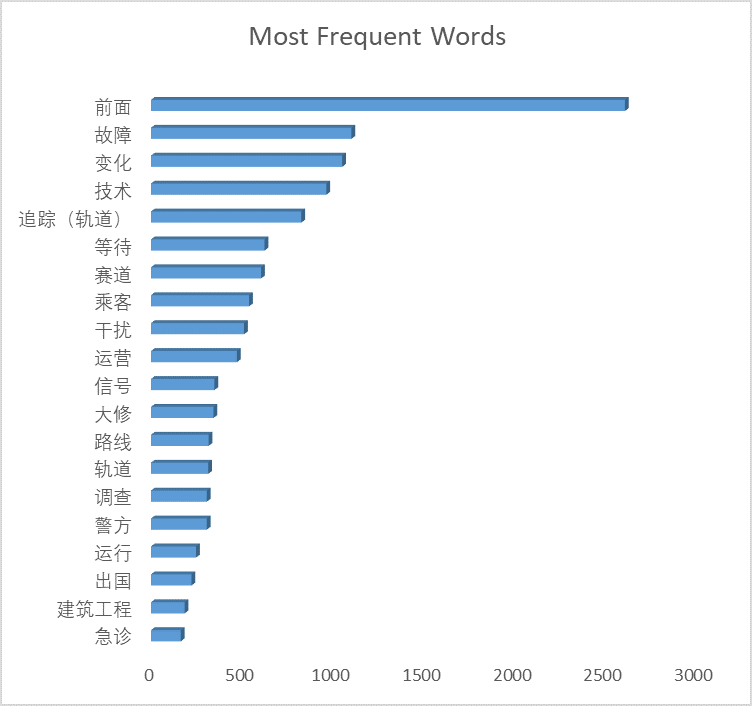
\includegraphics[width=0.5\textwidth]{image/freq.png}
	\caption{出现频数最高的20个词语}
	\label{fig7}
\end{figure}

从上图中我们发现,与语句分析部分相一致地,“前面”即由于前面列车晚点而造成的晚点出现次数最多,轨道变化、列车技术故障和警方调查仍是十分重要的晚点原因。同时,我们还发掘出更多原因细节,例如\textbf{“信号干扰”、“乘客急诊”、“建筑工程”}也常导致列车晚点。

\begin{figure}[H]
	\centering
	
\includegraphics[width=0.45\textwidth]{image/word_cloud.png}
	\caption{列车晚点原因词云}
	\label{fig8}
\end{figure}

通过对晚点原因的分析,我们得到了对于德国铁路运营管理者的一些启示:
\begin{itemize}
	\item[1.] 列车晚点现象可能存在“堆雪球”效应,一些班次列车的晚点不仅会影响该列车接下来线路上的站点,\textbf{还影响到其他班次的列车},特别是长途城际列车;相反,如果避免一些列车的晚点情况,还可能减少其他列车的延误。所以管理者应更加重视列车晚点问题,设法尽量避免晚点现象而减少成本,并提高乘客体验。
	\item[2.] 较多的轨道变化、运营延迟、进出延迟说明德铁在\textbf{轨道排程}方面也许有可以改进之处,若某些车站类似问题出现较多,甚至可以考虑扩建站台轨道来提高容量。
	\item[3.] \textbf{列车的技术故障及信号干扰}也是造成列车晚点的重要因素,管理者可以更深入地排查具体故障,并尝试对造成问题的主要技术做出改进。
\end{itemize}

\section{铁路交通网络分析}

在前文数据特点统计分析部分,我们发现长途城际列车(即I类列车)的晚点率远远超过,其他类型列车的晚点率。而且长途城际列车是在各大城市之间通行,R类和S类列车仅仅是区域内或城市内的交通,利用I类列车的这一特点,可以构建德国铁路交通网络,利用网络分析的方法研究数据集中各车站相互间的网络特点。

\subsection{总车流量静态网络分析}

首先筛选出I类列车的数据,保留下连通所选10个城市的数据,即列车路径中至少含有两个目标城市。以数据集中的10个城市车站为结点,I类列车的通路为边,结点的值设为通过该城市的I类列车总数,边的权重为在这条路线上经过的I类列车总数。例如ICE 10列车从法兰克福出发途经科隆,ICE 1536列车途经法兰克福和柏林,于是将法兰克福和科隆两个结点的边相连、将法兰克福和柏林两个结点的边相连,边的权重赋值为1,结点法兰克福的值为2,结点柏林和科隆的值为1。该网络为一个带权重的有向图或多个分开的有向子图。

按照这个规则,我们对数据集当天的I类列车总流量网络进行可视化,见附件中的交互式网页,图(\ref{fig9})仅为静态截图。

\begin{figure}[H]
	\centering
	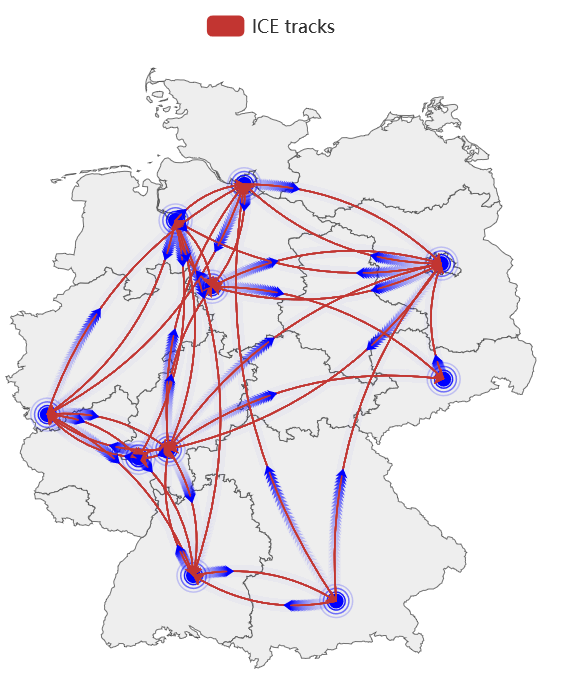
\includegraphics[width=0.5\textwidth]{image/graph1.png}
	\caption{I类列车总流量网络图}
	\label{fig9}
\end{figure}

我们关心网络中各种中心性的衡量,选取三种中心性作为指标:度中心性、邻近中心性和介中心性。其中度中心性(Degree Centrality)为一个结点所连接的边的数量,邻近中心性(Closeness Centrality)为一个结点到其他结点的平均最短距离,介中心性(Betweenness Centrality)为经过该结点的其他对结点的最短路径数量占所有其他对结点最短路径数的比例,它们的计算公式如下\citep{easley2010networks}:
\begin{align*}
& C_{D}(i)=k_{i}\\
& C_{c}(i)=\frac{n-1}{\sum_{j=1}^{n} d(i, j)}\\
& C_B(i) = \frac{2}{(n-1)(n-2)} \sum_{s<t \atop s, t \neq i} \frac{n_{s t}^{i}}{g_{s t}}
\end{align*}

在本数据集的情景下,度中心性体现了一个结点城市与其他城市间城际列车的多少,邻近中心性体现了该城市位于铁路网络中心的程度,而介中心性的值越高,表明该结点在连通其他大城市的过程中起到了重要作用,是铁路交通枢纽。这三种衡量指标都具有实际意义,所以对其进行分析是合理有效的。

于是使用Python的networkx包计算这三种中心性,得到的结果如表(\ref{tab3})所示。

\begin{table}[H]
	\centering
	\caption{列车总流量网络图各节点的中心性}
	\label{tab3}
	\begin{tabular}{l|ccccc}
		\hline
		& Berlin                         & Hannover                   & Stuttgart                      & Bremen                         & Hamburg                        \\ \hline
		Degree      & \cellcolor[HTML]{FFFFC7}57     & \cellcolor[HTML]{FFFFC7}58 & 19                             & 29                             & 35                             \\
		Closeness   & 0.2025                         & 0                          & 0.1423                         & \cellcolor[HTML]{FFFFC7}0.2638 & \cellcolor[HTML]{FFFFC7}0.2233 \\
		Betweenness & \cellcolor[HTML]{FFFFC7}0.6923 & 0.6428                     & 0.6428                         & 0.4736                         & \cellcolor[HTML]{FFFFC7}0.6923 \\ \hline
		& Mainz                          & Muechen                    & Frankfurt                      & Koeln                          & Dresden                        \\ \hline
		Degree      & 15                             & 16                         & \cellcolor[HTML]{FFFFC7}61     & 26                             & 10                             \\
		Closeness   & 0.1215                         & 0.0879                     & 0.2187                         & \cellcolor[HTML]{FFFFC7}0.2337 & 0.0694                         \\
		Betweenness & 0.5294                         & 0.409                      & \cellcolor[HTML]{FFFFC7}0.6923 & 0.6                            & 0.5294                        
	\end{tabular}
\end{table}

每种中心性数值最高的前三个城市已在表中用黄色背景标出,我们可以发现,长途城际列车进出量最多的三个城市是\textbf{法兰克福、汉诺威和柏林},它们的度中心性分别为61、58、57;整个网络的中心大致在靠近\textbf{不莱梅、科隆和汉堡}之间的地方,因为它们的邻近中心性值最大,分别为0.2638、0.2337和0.2233,其中汉诺威的邻近中心性为0,是因为它与其中某个城市不连通,距离为无穷而造成的;这10个城市中最为重要的交通枢纽为\textbf{柏林、汉堡和法兰克福},它们的介中心性取值最高,都为0.6923。

结合可视化图像分析,德国的长途铁路交通网络大致可以分为\textbf{北部、西南部和首都柏林三大长途铁路交通热点区域},北部的三大城市汉诺威、汉堡、不莱梅都有较强的中心性;西南部交通枢纽为法兰克福,科隆则是离境前往西欧其他国家的要道;柏林因为是德国首都,也拥有着来自全国各地的较多的流量。比较出人意料的是,德国东南部重镇、巴伐利亚州的首府慕尼黑的中心性却是10个城市中最低的之一。这似乎与现实生活经验有些出入,然而通过前文对数据集的分析,我们已经可以看出端倪:慕尼黑的数据中S类列车占约$80\%$,仅有很少的一部分是I类列车。这与我们在网络分析中得到的结果一同说明,慕尼黑在巴伐利亚州的区域内交通较为发达,而对于长途的城际交通则在显得不足。

\subsection{列车延误时长静态网络分析}

接下来,我们按照类似的方法构建晚点列车的网络图,以数据集中的10个城市车站为结点,晚点的I类列车的通路为边。但此时我们更关心长途列车晚点的总时间,而不是晚点的列车次数,所以结点的值设为通过该城市的所有晚点I类列车延误时间总和,而边的权重仍为在这条路线上经过的晚点I类列车总数。例如ICE 10列车从法兰克福出发途经科隆,且在法兰克福至科隆途中晚点了15分钟,于是将法兰克福和科隆两个结点的边相连,并将边赋值为1,结点法兰克福和科隆的值为15。于是同样可以画出延误列车网络的可视化图形:

\begin{figure}[H]
	\centering
	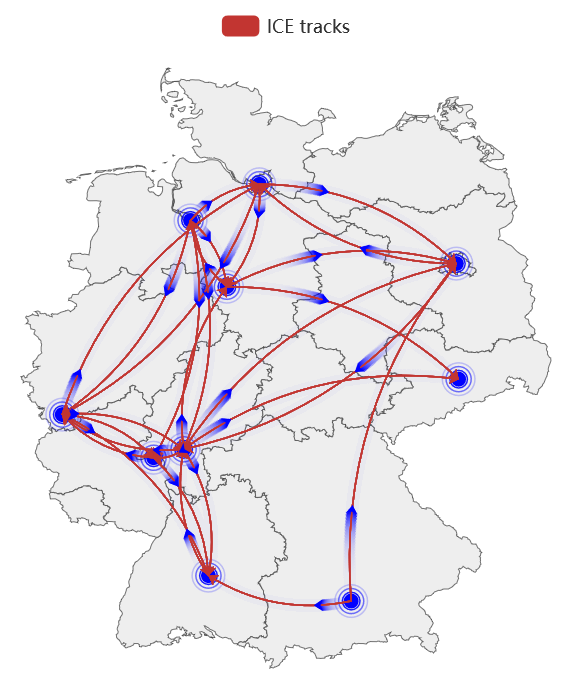
\includegraphics[width=0.5\textwidth]{image/graph2.png}
	\caption{晚点I类列车流量网络图}
	\label{fig10}
\end{figure}

晚点列车网络图的三种中心性取值为:

\begin{table}[H]
	\centering
	\caption{晚点列车流量网络图各节点的中心性}
	\label{tab4}
	\begin{tabular}{l|ccccc}
		\hline
		& Berlin                        & Hannover & Stuttgart                      & Bremen                         & Hamburg                     \\ \hline
		Degree      & \cellcolor[HTML]{FFFFC7}340   & 286      & 27                             & 218                            & \cellcolor[HTML]{FFFFC7}336 \\
		Closeness   & 0                             & 0.125    & \cellcolor[HTML]{FFFFC7}0.3194 & 0.0694                         & 0.1527                      \\
		Betweenness & \cellcolor[HTML]{FFFFC7}0.547 & 0.474    & \cellcolor[HTML]{FFFFC7}0.547  & 0.3232                         & 0.5079                      \\ \hline
		& Mainz                         & Muechen  & Frankfurt                      & Koeln                          & Dresden                     \\ \hline
		Degree      & 115                           & 28       & \cellcolor[HTML]{FFFFC7}457    & 209                            & 54                          \\
		Closeness   & 0.0277                        & 0        & \cellcolor[HTML]{FFFFC7}0.4027 & \cellcolor[HTML]{FFFFC7}0.2916 & 0                           \\
		Betweenness & 0.5079                        & 0        & \cellcolor[HTML]{FFFFC7}0.5925 & \cellcolor[HTML]{FFFFC7}0.547  & 0.5                        
	\end{tabular}
\end{table}

每种中心性数值最高的前三个城市已在表中用黄色背景标出,可以清楚地观察到\textbf{法兰克福、科隆、斯图加特所在的德国西南部是列车晚点的“重灾区”},晚点列车网络的中心毫无疑问地落在德国西南地区,汉堡所在的德国北部和柏林也有较长的延误时间,但没有西南部严重。由于它们都是前文提到的交通密集的地区,柏林和汉堡有些许延误是可以理解的,但西南地区的情况则过于糟糕,是交通网络中的一大问题。

根据网络的邻接矩阵(adjacency matrix),列车晚点总时长最多的三条路径为:柏林至法兰克福,共延迟124分钟;汉堡至汉诺威,共延迟122分钟;不莱梅至汉堡,共延迟105分钟。由此,德国北部地区的列车晚点也是不容忽视的问题,汉堡、汉诺威、不莱梅三城的铁路距离较短,它们的总延迟时间却与柏林至法兰克福这一从东北至西南横穿德国的线路相近,德铁运营者也许需要\textbf{更加深入地探查北部的这几段铁路},结合具体情况了解晚点原因,并实施合适的对策。

用晚点列车网络的度中心性除以总列车网络的度中心性,得到各个城市每趟晚点列车的平均延误时间。我们发现,除去上述的交通密集城市,紧邻法兰克福西部的\textbf{美因茨的平均延误时间达到了7.67分钟},高于法兰克福的平均延误时长,位列所有城市的第三!如果说法兰克福和科隆是由于处在交通要道,车流量大而导致总延误时长较长,还情有可原,但美因茨自身的车流量并不大,就更能反映出德国西南部铁路交通存在一定的问题,这种延误问题不仅在枢纽城市,还\textbf{波及到其他中小城市}。


\subsection{动态网络分析}

在分析了一天中总体的所有列车和晚点列车的网络后,我们进一步考虑时间因素,类似数据特点统计分析部分,将一天分为不同时间段,研究随时间的推进,不同时间段网络的动态变化。由于单独一个小时内途经各城市的I类列车数量过少,我们将时间按照4个小时的区间划分,从当天最早的一班I类火车开始,至最晚的一班,分为9-12时、10-13时、…、20-23时12个时段,分别对各个时段建立列车流量网络,并分析其随时间的变化规律。使用pyecharts画出的动态交互时间轴网络图见附件中的网页文件,图(\ref{fig11})为12个时段中较为典型的时段网络截图。

\begin{figure}[H]
	\centering
	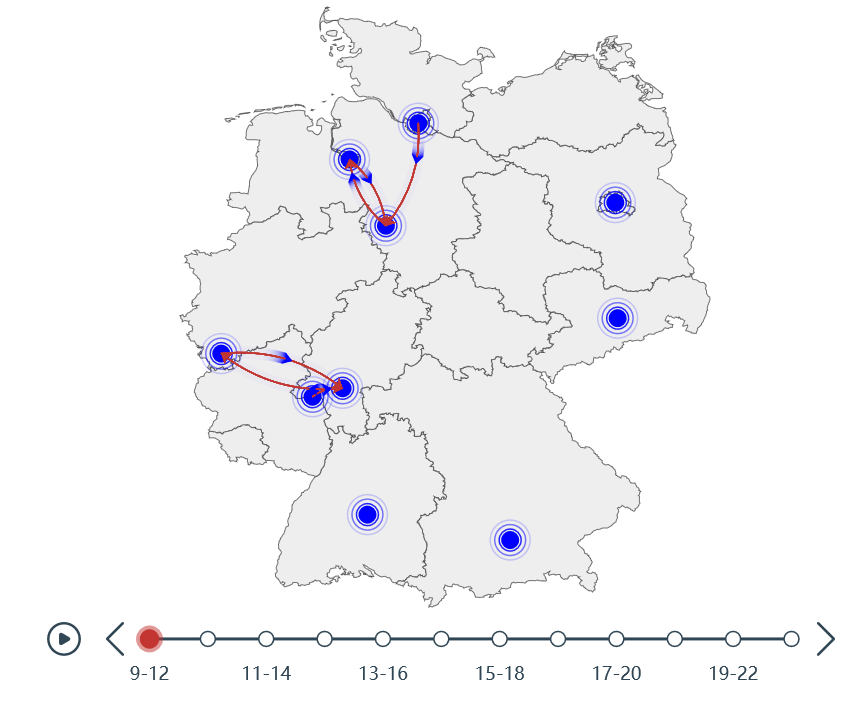
\includegraphics[width=0.3\textwidth]{image/graph31.png}
	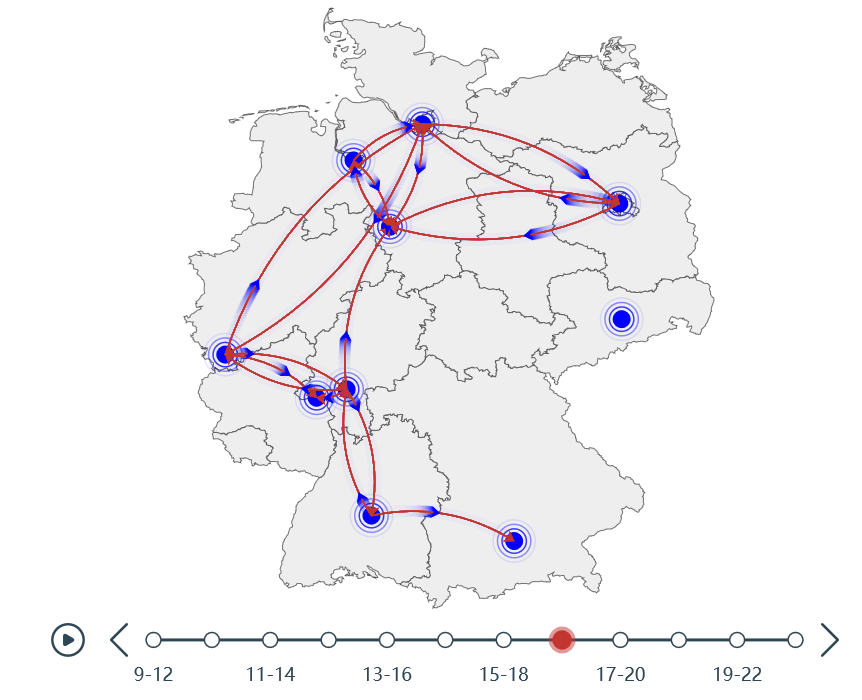
\includegraphics[width=0.3\textwidth]{image/graph32.png}
	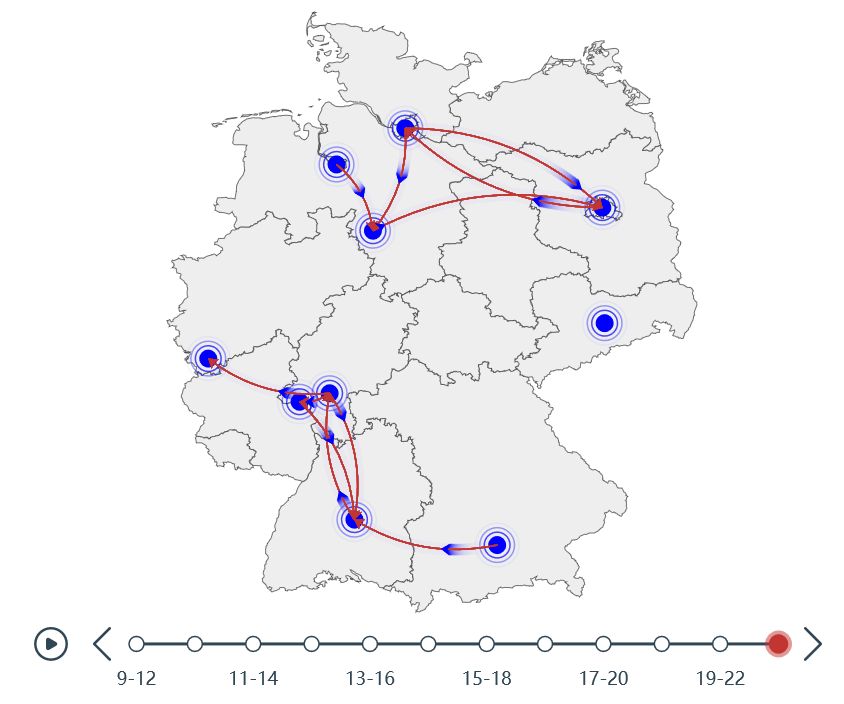
\includegraphics[width=0.3\textwidth]{image/graph33.png}
	\caption{一天中不同时段I类列车流量网络图}
	\label{fig11}
\end{figure}

总体而言一天的列车流量从上午的低谷增高,至深夜再次减少。左图为最早的9-12时列车流量,可以看出此时的长途列车较少,仅有交通密集区北部和西南部的城市构成两个三角结构(triadic);之后列车数量逐渐增多,各分区内的交通更加密集,同时分区之间也有了联系,一张连通的交通网络图逐渐成型,中图为16-19时的列车流量,此时为一天中各区域连通性最高的时段;右图为20-23时的列车流量,此时交通量已经减少,但各分区内仍有相当数量的列车运行,总体流量要多于上午最早时段的车流情况。

而对于这12个时段的列车晚点率,从最初的上午时间就处于较高的水平,\textbf{到中午11-14时达到一天的高峰},约为$73.17\%$,之后则平缓下降,直至深夜的最低点$49.84\%$。这一随时间逐步下降的趋势与前文数据特点分析的结果一致,而网络分析的结果将前文得到的中午11时、13时及晚间18时、21时这四个流量高峰更精确地锁定在中午时段,管理者为了更高效地降低列车晚点数量,\textbf{应注重于中午时段的高峰}。

总之,在对静态和动态的铁路网络分析后,我们发现了一些新的管理启示:
\begin{itemize}
	\item[1.] 主要的长途铁路交通密集区有三个:北部的汉堡、汉诺威、不莱梅三城;西南部的法兰克福和科隆;首都柏林。其中\textbf{受到晚点问题影响最严重的是德国西南地区}。
	\item[2.] 晚点问题最严重的路段为柏林至法兰克福、汉堡至汉诺威、不莱梅至汉堡,其中\textbf{北部的两段线路应更加重视},因为更可能通过人为措施进行改善,而不是系统性的误差。
	\item[3.] 每天的\textbf{中午时段(约11-14时)是列车流量和晚点率都较高的时段},应重点关注。
\end{itemize}


\section{总结与讨论}

在最后这一部分,我们将对本文德国铁路数据的分析方法、过程进行概述,讨论数据分析结果对德铁运营者的管理启示,并尝试提出可能的改进方案。之后指出本文分析中未涉及到的方面,揭示可能的进一步研究方向,最后以精简的总结结束全文。

\subsection{管理启示与改进应用}

在前文的数据集统计分析、晚点原因文本分析和铁路交通网络分析中,我们都发现了数据或多或少的一些特点,在此结合我们的心智模型,即在现有信息下降低列车晚点数量、最优化铁路运营者收益和乘客服务体验,归纳出几条向德国铁路公司提出的运营管理启示,并根据本文数据集提供的信息提出现实的改进建议。主要的管理启示和改进建议如下:
\begin{itemize}
	\item[1.] \textbf{从各城市车站角度},重点关注网络分析部分提到的西南部、北部和柏林交通区的城市,针对不同分区深入了解具体情况,根据不同地区的特色制定不同方案。例如,西南地区连通西欧各国的科隆列车晚点问题较为严重,可以考虑新建其他出境线路来引流,而同属西南地区的法兰克福既是国内的铁路枢纽,在市区附近又有国际机场,可以在考察主火车站容量后考虑适当增加站台和轨道来缓解晚点问题。
	\item[2.] \textbf{从长短途列车角度},虽然长途列车的晚点率显著更高,且一旦晚点一般延迟时间就较长,但短途列车的晚点问题仍然重要。在晚点原因中我们知道前方列车晚点是出现次数最多的原因之一,而这一原因更可能出现在短途列车上,再加上S类列车涉及到城市内交通的情况,可能出现多频次、短时间的晚点现象,这就需要运营者在让晚点影响到下一趟列车和改变线路之间做出权衡,要求德铁工作人员有较高的实时系统优化能力。
	\item[3.] \textbf{从一天中不同时间段的角度},结合统计分析和网络分析的结果,我们知道每天的中午时段(约11-14时)是列车流量和晚点率都较高的时段。管理者可以考虑在高峰时段增派工作人员来应对晚点情况,也可以考虑将一些班次列车的发车时间适当提前或延后,来使高峰平缓,进而减少晚点现象。但后者就涉及到乘客对列车到达时间的需求和调整时间对铁路公司自身的其他影响,由于我们没有掌握相关信息,所以这条建议仅作为可能的假设。
	\item[4.] \textbf{从晚点原因角度},较多的轨道变化、运营延迟、进出延迟说明德铁在轨道排程方面有可以提高的空间,若某些车站类似问题出现较多,甚至可以考虑扩建站台轨道来提高容量。列车的技术故障及信号干扰也是造成列车晚点的重要因素,管理者可以更深入地排查具体故障,并尝试对造成问题的主要技术做出改进。
\end{itemize}

\subsection{进一步研究}

尽管本文对德国铁路数据的分析已经对管理有了现实的启示,但仍有一些不足之处和未来研究的可能方向。

首先,本文的数据集仅有一天的列车数据,一些列车的晚点可能是特殊情况,进而对分析的信度产生影响。由于每天的列车班次基本不会改变,所以如果\textbf{收集更多天数的列车数据},将会得到在统计意义上更加可靠的结果。

其次,该数据集很容易让人想到使用\textbf{面板回归}(Panel Data Regression)方法进行分析,例如也许有各个车站相同且随时间变化的影响晚点的因素,或是不随时间变化却每个车站不同的因素。而在收集更多天数列车数据的情况下,甚至可以考虑\textbf{时间序列分析}(Time Series Analysis)的分析方法。但我们认为衡量晚点情况的因变量无法很好地确定,无论是晚点列车数量、晚点率、晚点总时长都不是十分恰当,且要想找到具有实际经济意义的自变量非常困难,甚至可能出现因果转置(Inverse Causality)的问题,所以我们最终没有采用上述两种分析方法。若后人发现了回归方法对于数据可解释的逻辑,那么回归分析和时间序列分析不失为一个有趣的研究方向。

然而需要说明的是,收集更多天数的列车数据增加了数据集的维度,本文中已有的车站、列车、一天内的时间三个维度已经使得数据的切块和处理有很大的难度,若再加入一个维度,在使数据更丰富的同时无疑会带来\textbf{更大的挑战}。

在微观方面,本文网络分析部分将研究角度缩小到I类列车,可以更进一步地研究单独一列ICE列车,根据它的路径和发车时间,尝试\textbf{预测其晚点情况}。但本文数据集中仅包含了德国10个较为重要的城市,长途城际列车绝大多数是从其中一城发往另一城,极少出现数据集中三个及以上城市出现在同一列车线路上的情况,这样我们无法得知列车沿途其他站点的到站时间等信息,若要进行预测则效果必然不佳,所以没有进行类似的尝试。

最后,在车站的运营管理方面也有可以继续研究的问题。本文的数据集中是包含了列车进站时停靠的站台编号信息的,但我们更多地是对数据进行描述性分析,没有用到停靠站台信息,其实可以更深入地讨论铁路运营中的优化问题。如果要对其进行发掘,可以通过不同时刻站台的使用率,考虑列车晚点时的车站站台轨道更改排程,是一个\textbf{涉及决策、排队等方面的综合性运营管理问题}。

\subsection{总结}

本文对德国铁路一天内列车晚点数据进行分析,首先在车站、列车类型和一天内的时间段三个角度对数据集进行切块处理,分析列车总流量、晚点列车数量、延误时长等指标在不同角度呈现出的特点。接着使用分词、统计词频、构建词云等文本分析技术,提取主要的晚点原因。然后使用加工后的数据构建列车总流量、晚点总时长的交通网络图,利用网络分析方法中的中心性作为指标衡量车流量及延误情况,最后构建动态交通网络,探究一天内不同时段的交通流特点。

通过上述分析,我们发现数据的诸多隐藏特点,并结合假定的心智模型提出一些具有现实指导意义的管理启示,我们认为这些建议对德国铁路公司管理者有较大的帮助。同时,本文还指出为了控制德铁列车晚点现象,减少德铁公司的运营成本并提高德铁列车乘客的服务体验,可能的进一步研究方向,对未来研究相关问题的学者有指导和借鉴意义。

\section*{致谢}

我曾于2019年秋季学期在德国度过了一个交换学期,当时我就对德国的铁路系统有着浓厚的兴趣,它既有胜过国内的事实列车信息更新系统,也有本文提到的饱受诟病的晚点问题,其便捷与麻烦之处本人都亲身体验过许多次,可以说我是怀有感情地写作这篇课程报告。所以首先得感谢清华大学经济管理学院的毛波老师,是毛老师的《商务数据分析》课程使得我有机会利用所学知识认真探究我感兴趣的话题;同时也需要感谢Kaggle网站社区,提供了刚好适用我所打算分析的情景的数据集,省去了爬取数据的时间。最后,我十分享受完成这篇文章时的每一步,从构思、写Python代码分析、数据可视化到文章的撰写和修改,希望能为我这门专业课以及整个大三学年画上一个完美的句号。

~\\

%\newpage
\nocite{*}
\bibliography{paper1}

\newpage
\appendix
\appendixpage
\addappheadtotoc

所打包上传的文件中包括以下部分:
\begin{itemize}
	\item 原始数据集,保存在$DB\_data$文件夹中,包含10个$csv$文件。
	\item 程序需要用到的其他数据,保存在$data$文件夹中。
	\item 分析时用到的Python程序文件,$util.py$为对数据的清洗和预处理,$text.py$为晚点原因文本分析,$network.py$为构建列车交通网络并计算中心性,$total\_graph.py$、$delayed\_graph.py$和$timeline.py$是对交通网络的可视化,分别为总流量网络、晚点列车网络和一天中不同时间段的交通网络。
	\item 交通网络可视化的html文件,分别是$total\_track\_graph.html$、$delayed\_track\_graph.html$和$timeline\_map.html$。
\end{itemize}





\end{document}
